\documentclass[11pt,a4paper]{article}
%\usepackage[utf8]{inputenc}
%\usepackage[ascii]{inputenc}
%\usepackage{geometry}
\usepackage[margin=0.7in]{geometry}
\usepackage[dvipsnames]{xcolor}
\usepackage{textcomp}
\usepackage{graphicx}
\usepackage{caption}
\usepackage{subcaption}
\usepackage{amssymb}
\usepackage{amsmath}
\usepackage{tikz}

\begin{document}
\title{Résumé \& Méthodes chapitre III: Signaux Numériques}
\maketitle

\section{Signal numérique: Défintion}
\vspace{0.3cm}
\begin{center}
\fbox{
\textbf{Signal numérique =  Codage + \'Echantillonnage}
}
\end{center}
\vspace{0.3cm}
\section{Codage}
\underline{\textbf{Codage }}: Mode de répresentation discret de l'amplitude caractérisé par des \textbf{quantas} et une \textbf{dynamique de codage}\\

\vspace{0.3cm}

\begin{center}
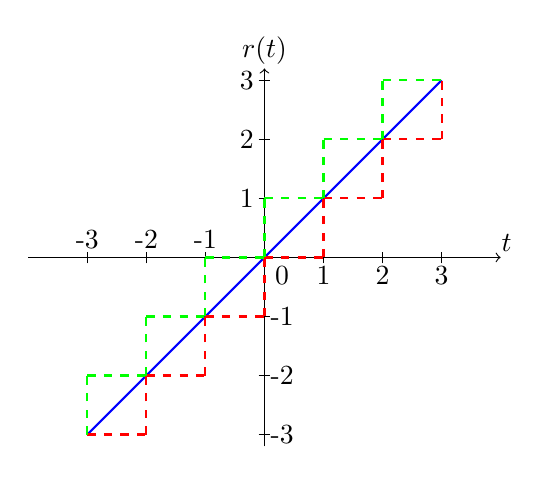
\begin{tikzpicture}
\begin{scope}[scale = 0.75]
\draw[->] (-4,0)-- (4,0);
\draw (0.3,-0.3) node {0};
\draw[->] (0,-3.2)-- (0,3.2);
\draw (4.1,0.25) node {$t$};
\draw (0,3.5) node {$r(t)$};

\draw (1,-0.1)-- (1,0.1);
\draw (1.0,-0.3) node {1};
\draw (2,-0.1)-- (2,0.1);
\draw (2.0,-0.3) node {2};
\draw (3,-0.1)-- (3,0.1);
\draw (3.0,-0.3) node {3};

\draw (-1,-0.1)-- (-1,0.1);
\draw (-1.0,0.3) node {-1};
\draw (-2,-0.1)-- (-2,0.1);
\draw (-2.0,0.3) node {-2};
\draw (-3,-0.1)-- (-3,0.1);
\draw (-3.0,0.3) node {-3};

\draw (-0.1,1)-- (0.1,1);
\draw (-0.3,1) node {1};
\draw (-0.1,2)-- (0.1,2);
\draw (-0.3,2) node {2};
\draw (-0.1,3)-- (0.1,3);
\draw (-0.3,3) node {3};

\draw (-0.1,-1)-- (0.1,-1);
\draw (0.3,-1) node {-1};
\draw (-0.1,-2)-- (0.1,-2);
\draw (0.3,-2) node {-2};
\draw (-0.1,-3)-- (0.1,-3);
\draw (0.3,-3) node {-3};

%r(t)
\draw[thick,blue] (-3,-3)-- (3,3);

\draw[thick,dashed,red] (-3,-3)-- (-2,-3);
\draw[thick,dashed,red] (-2,-3)-- (-2,-2);
\draw[thick,dashed,red] (-2,-2)-- (-1,-2);
\draw[thick,dashed,red] (-1,-2)-- (-1,-1);
\draw[thick,dashed,red] (-1,-1)-- (-0,-1);
\draw[thick,dashed,red] (-0,-1)-- (-0,-0);
\draw[thick,dashed,red] (-0,-0)-- (1,-0);
\draw[thick,dashed,red] (1,0)-- (1,1);
\draw[thick,dashed,red] (1,1)-- (2,1);
\draw[thick,dashed,red] (2,1)-- (2,2);
\draw[thick,dashed,red] (2,2)-- (3,2);
\draw[thick,dashed,red] (3,2)-- (3,3);

\draw[thick,dashed,green] (-3,-2)-- (-2,-2);
\draw[thick,dashed,green] (-3,-3)-- (-3,-2);
\draw[thick,dashed,green] (-2,-1)-- (-1,-1);
\draw[thick,dashed,green] (-2,-2)-- (-2,-1);
\draw[thick,dashed,green] (-1,-0)-- (-0,-0);
\draw[thick,dashed,green] (-1,-1)-- (-1,0);
\draw[thick,dashed,green] (-0,1)-- (1,1);
\draw[thick,dashed,green] (0,0)-- (0,1);
\draw[thick,dashed,green] (1,2)-- (2,2);
\draw[thick,dashed,green] (1,1)-- (1,2);
\draw[thick,dashed,green] (2,3)-- (3,3);
\draw[thick,dashed,green] (2,2)-- (2,3);
\end{scope}
\end{tikzpicture}\\
\vspace{0.5cm}
\underline{Exemple}: 2 possibilités de codage d'une fonction rampe par arrondi (vert) et par troncature (rouge) sur 6 quantas/échelons d'échantillonnage et une gamme de 6 unités
\end{center}

\newpage
\section{\'Echantillonnage}
\underline{\textbf{ \'Echantillonnage} } : "L’échantillonnage consiste à représenter un signal fonction du temps $x(t)$ par ses
valeurs $x(nT_e)$ à des instants multiples entiers d’une durée $T_e$, appelée \textbf{période d’échantillonnage}."\\
\footnotesize {M. Bellanger}


\subsection{Peigne de Dirac}
\normalsize L'opération d'échantillonnage s'appuie sur la distribution appelée "peigne de Dirac"\\ 

 \[ u_{T_e}(t) = \sum_{n = -\infty}^{\infty} \delta(t-nT_e) \]\\
 
 Et par suite, soit $s(t)$ un signal continu,
 
\[\boxed{x(nT_e) = x(t) \cdot u_{T_e}(t)}\]

\subsection{Impact sur le spectre}
Partons d'un signal continu et de son spectre :\\
\vspace{0.5cm}\\
\begin{center}
\begin{tikzpicture}
\begin{scope}[scale=0.6]
	\draw[->] (-5,0)-- (5,0);
%\draw (-0.3,-0.3) node {0};
\draw[->] (0,-3)-- (0,3);
\draw (5.3,0.25) node { $t$};
\draw (0,3.5) node {$u_{T_{e}}(t)x(t)$};
%\draw (4.5,-0.3) node {1};

\draw[domain=-4.9:4.9,color=blue,samples=160] plot (\x,{2*(0.55*cos(2*\x r)+ 0.45*cos(2*2*(\x+3.14/12) r))});

%\draw[domain=-4.9:4.9,color=blue,samples=16] plot[ycomb] (\x,{2*(0.55*cos(2*\x r)+ 0.45*cos(2*2*(\x+3.14/12) r))});

\end{scope}

\begin{scope}[scale=0.6,xshift=15 cm]
	\draw[->] (-5,0)-- (5,0);
\draw[->] (0,0)node[below] {0} -- (0,3);
\draw (5.2,0.25) node { $\nu$};
\draw (0,3.5) node { $|X(\nu)|$};
%\draw (4.5,-0.3) node {1};


\draw[thick,blue] (1.05,0)-- (1.05,2.5*0.55);
\draw[thick,blue] (2.05,0)-- (2.05,2.5*0.45);
\draw (2.1,-0.8) node { $\frac{2}{\pi}$};
\draw (1.1,-0.8) node { $\frac{1}{\pi}$};

\draw[thick,blue] (-1.05,0)-- (-1.05,2.5*0.55);
\draw[thick,blue] (-2.05,0)-- (-2.05,2.5*0.45);
\draw (-2.1,-0.8) node {  $-\frac{2}{\pi}$};
\draw (-1.1,-0.8) node {$-\frac{1}{\pi}$};
\end{scope}

\end{tikzpicture}
\end{center}

\'Echantillonnons le signal pour comprendre l'impact  de cette opération sur le spectre\\
\vspace{0.5cm}\\
\begin{center}
\begin{tikzpicture}
\begin{scope}[scale=0.6]
	\draw[->] (-5,0)-- (5,0);
%\draw (-0.3,-0.3) node {0};
\draw[->] (0,-3)-- (0,3);
\draw (5.3,0.25) node { $t$};
\draw (0,3.5) node { $u_{T_{e}}(t)x(t)$};
%\draw (4.5,-0.3) node {1};

\draw[domain=-4.9:4.9,color=cyan,samples=16] plot (\x,{2*(0.55*cos(2*\x r)+ 0.45*cos(2*2*(\x+3.14/12) r))});

\draw[dotted,domain=-4.9:4.9,color=blue,samples=160] plot (\x,{2*(0.55*cos(2*\x r)+ 0.45*cos(2*2*(\x+3.14/12) r))});

\draw[dashed,domain=-4.9:4.9,color=blue,samples=16] plot[ycomb] (\x,{2*(0.55*cos(2*\x r)+ 0.45*cos(2*2*(\x+3.14/12) r))});

\end{scope}

\begin{scope}[scale=0.6,xshift=15cm]
	\draw[->] (-6.5,0)-- (6.5,0);
\draw (-0,-0.3) node {\scriptsize 0};
\draw[->] (0,0)-- (0,3);
\draw (7.2,0.25) node {$\nu$};
\draw (0,3.5) node { $|X(\nu)|$};
%\draw (4.5,-0.3) node {1};


\draw[thick,blue] (1.05,0)-- (1.05,2.5*0.55);
\draw[thick,blue] (2.05,0)-- (2.05,2.5*0.45);
\draw (2.1,-0.6) node { $\frac{2}{\pi}$};
%\draw (1.1,-0.4) node {$\frac{1}{\pi}$};

\draw[thick,blue] (-1.05,0)-- (-1.05,2.5*0.55);
\draw[thick,blue] (-2.05,0)-- (-2.05,2.5*0.45);
%\draw (-2.1,-0.4) node {$-\frac{2}{\pi}$};
%\draw (-1.1,-0.4) node {$-\frac{1}{\pi}$};


%replica 1
\draw[thick,cyan] (5.05,0)-- (5.05,2.5*0.55);
\draw[thick,cyan] (6.05,0)-- (6.05,2.5*0.45);
%\draw (5.1,-0.4) node {$\frac{5}{\pi}$};
%\draw (6.1,-0.4) node {$\frac{6}{\pi}$};

\draw[thick,cyan] (3.05,0)-- (3.05,2.5*0.55);
\draw[thick,cyan] (2.08,0)-- (2.08,2.5*0.45);
%\draw (3.1,-0.4) node {$\frac{3}{\pi}$};
%\draw (2.1,-0.4) node {$\frac{1}{\pi}$};
\draw (4.1,-0.8) node { $\frac{4}{\pi}$};


%replica 2
\draw[thick,cyan] (-5.05,0)-- (-5.05,2.5*0.55);
\draw[thick,cyan] (-6.05,0)-- (-6.05,2.5*0.45);
%\draw (-5.1,-0.4) node {$-\frac{5}{\pi}$};
%\draw (-6.1,-0.4) node {$-\frac{6}{\pi}$};

\draw[thick,cyan] (-3.05,0)-- (-3.05,2.5*0.55);
\draw[thick,cyan] (-2.08,0)-- (-2.08,2.5*0.45);
%\draw (-3.1,-0.4) node {$-\frac{3}{\pi}$};
%\draw (2.1,-0.4) node {$\frac{1}{\pi}$};
\draw (-4.1,-0.8) node { $-\frac{4}{\pi}$};
\end{scope}
\end{tikzpicture}
\end{center}

\newpage
\section{Critère de Shannon \& Repliement spectral}
\vspace{0.2cm}
\fbox{
\begin{minipage}{\textwidth}
\underline{\textbf{Critère de Shannon :}}
Pour échantillonner un signal sans perte d'information, il faut que la \textbf{fréquence d'échantillonnage soit deux fois supérieure à la fréquence maximale présente dans le signal} $\rightarrow$ $\nu_e > 2 \nu_{max}$
\end{minipage}
}
\\
\vspace{0.4cm}\\
De façon générale, \\
\vspace{0.2cm}\\
\begin{tikzpicture}
\begin{scope}[scale=0.7]
	\draw[->] (-5,0)-- (5,0)node[right] {$\nu$};
\draw[->] (0,0)node[below] { 0} -- (0,3)node[above] { $|X(\nu)|$};

\draw[blue,thick](-1,0)--(-0.5,1)--(0.5,1)--(1,0);
\end{scope}

\begin{scope}[scale=0.7,xshift=12cm]
	\draw[->] (-5,0)-- (5,0)node[right] {$\nu$};
\draw[->] (0,0)node[below] { 0} -- (0,3)node[above] { $|X(\nu)|$};

\draw[blue,thick](-1,0)node[below,black]{$-\nu_{max}$}--(-0.5,1)--(0.5,1)--(1,0)node[below,black]{$\nu_{max}$};
\draw[blue,thick](-1+3,0)--(-0.5+3,1)--(0.5+3,1)--(1+3,0);
\draw[blue,thick](-1-3,0)--(-0.5-3,1)--(0.5-3,1)--(1-3,0);
\draw[dashed] (3,0) node[below]{$\nu_e$} --(3,1);
\draw[dashed] (-3,0) node[below]{$-\nu_e$} --(-3,1);
\end{scope}
\end{tikzpicture}
\\
\vspace{0.1cm}\\
Or si $\nu_e < 2 \nu_{max}$\\
\vspace{0.1cm}\\
\begin{tikzpicture}
\begin{scope}[scale=0.7]
	\draw[->] (-5,0)-- (5,0)node[right] {$\nu$};
\draw[->] (0,0)node[below] { 0} -- (0,3)node[above] { $|X(\nu)|$};

\draw[blue,thick](-1,0)--(-0.5,1)--(0.5,1)--(1,0);
\end{scope}

\begin{scope}[scale=0.7,xshift=12cm]
	\draw[->] (-5,0)-- (5,0)node[right] {$\nu$};
\draw[->] (0,0)node[below] { 0} -- (0,3)node[above] { $|X(\nu)|$};

\draw[blue,thick](-1,0)node[below,black]{$-\nu_{max}$}--(-0.5,1)--(0.5,1)--(1,0)node[below,black]{$\nu_{max}$};
\draw[blue,thick](-1+1.5,0)--(-0.5+1.5,1)--(0.5+1.5,1)--(1+1.5,0);
\draw[blue,thick](-1-1.5,0)--(-0.5-1.5,1)--(0.5-1.5,1)--(1-1.5,0);
\draw[dashed] (1.5,0) --(1.5,1)node[above]{$\nu_e$};
\draw[dashed] (-1.5,0) --(-1.5,1)node[above]{$-\nu_e$};
\end{scope}
\end{tikzpicture}
\\
\vspace{0.3cm}\\
\textbf{Donc si on ne respecte pas le critère de Shannon on obtient du repliement spectral.}\\
\vspace{0.3cm}\\
\fbox{
\begin{minipage}{\textwidth}
\underline{\textbf{Repliement spectral :}}
Si on ne respecte pas le critère de Shannon, Le spectre initial et ses repliques dues à l'échantillonnage s'entrecroisent
\end{minipage}
}
 


\end{document}